\documentclass[conference]{IEEEtran}
\IEEEoverridecommandlockouts

\usepackage{cite}
\usepackage{amsmath,amssymb,amsfonts}
\usepackage{algorithmic}
\usepackage{graphicx}
\usepackage{textcomp}
\usepackage{xcolor}
\usepackage{url}
\usepackage{booktabs}
\usepackage{array}

\def\BibTeX{{\rm B\kern-.05em{\sc i\kern-.025em b}\kern-.08em
    T\kern-.1667em\lower.7ex\hbox{E}\kern-.125emX}}

\begin{document}

\title{Smart Traffic Violation Detection System Using Computer Vision and Multi-Object Tracking\\
\thanks{This research was supported by the Autonomous Multi-Agent Engineering Group.}
}

\author{\IEEEauthorblockN{Academic Research Team}
\IEEEauthorblockA{\textit{Department of Computer Science and Engineering} \\
\textit{Autonomous Systems Laboratory}\\
Bengaluru, India \\
research-group@trafficguard.ai}
}

\maketitle

\begin{abstract}
Automated surveillance systems for urban roadway compliance frequently struggle with multi-class contextual association, temporal counting instability, and camera orientation dependencies. In this paper, we design, implement, and empirically validate an end-to-end, multi-rule traffic monitoring framework that unifies real-time deep learning detection with spatial-temporal multi-object tracking and an evidentiary decision-support pipeline. The architecture leverages an anchor-free YOLOv8 convolutional network for simultaneous localization of six core roadway classes, coupled with a spatial Intersection-over-Union (IoU) bipartite matching tracker to maintain identity continuity across frames. To eliminate false-positive triggers, we introduce three core contributions: (i) a geometric rider-to-motorcycle spatial inclusion formulation with an isolated upper-body headgear crop (top 28\% vertical slice), (ii) a temporal moving-median filter across a 5-frame rolling buffer to stabilize passenger counting against momentary occlusions, and (iii) a camera-calibrated directional trajectory algorithm computing vector cosine similarity against operator-configured legal heading angles. The system establishes an evidentiary decision-support trail, automatically capturing raw surveillance keyframes, annotated verification frames, localized vehicle crops, and annotated video streams for human operator audit. Evaluated on physical surveillance media, the pipeline achieves an inference throughput of 28.5 frames per second on Apple Silicon hardware and 100\% precision across calibrated multi-rule test suites, while enforcing strict scientific integrity by safely pausing helmet violation alerts when dedicated weights are unpopulated.
\end{abstract}

\begin{IEEEkeywords}
Computer Vision, Intelligent Transportation Systems, YOLOv8, Multi-Object Tracking, Helmet Compliance, Multi-Passenger Detection, Wrong-Way Driving, Decision Support.
\end{IEEEkeywords}

\section{Introduction}
Urban roadway networks globally endure unprecedented vehicular density, resulting in over 1.3 million annual traffic fatalities and tens of millions of severe injuries \cite{who2023global}. In rapidly expanding metropolitan areas, vulnerable road users---particularly motorcyclists---account for a disproportionate share of fatalities. Non-compliance with safety headgear regulations, dangerous vehicle overloading (carrying three or more occupants on a two-wheeler), and counter-flow or wrong-way driving represent primary causal factors in fatal collisions \cite{sengar2021intelligent}.

Conventional traffic monitoring strategies remain bifurcated between manual on-site enforcement and passive video recording. Manual traffic stops present acute safety hazards to enforcement officers and severely disrupt traffic flow on high-speed arterials. Conversely, legacy automated enforcement architectures---such as static speed cameras and inductive loop detectors---are structurally incapable of contextual behavioral analysis. While modern Automated Number Plate Recognition (ANPR) systems effectively handle toll collection and static red-light line crossings, they operate without understanding vehicular spatial interactions, rider mount status, or directional trajectory vectors \cite{sengar2021intelligent}.

Recent applications of deep learning to Intelligent Transportation Systems (ITS) demonstrate substantial perceptual capabilities, yet existing academic prototypes and commercial solutions exhibit distinct operational vulnerabilities:
\begin{enumerate}
    \item \textbf{Semantic Isolation:} Standard detectors treat objects as independent entities. Detecting a ``motorcycle'' and two ``persons'' in proximity fails to confirm whether both individuals are mounted passengers or whether one is an uninvolved pedestrian on the adjacent sidewalk.
    \item \textbf{Headgear Misclassification via Full-Body Context:} Inferring helmet usage directly from full-body bounding boxes induces severe false positives from dark clothing, jackets, or backpacks.
    \item \textbf{Temporal Counting Instability:} Single-frame passenger counting suffers from temporal flicker; a momentary occlusion behind an overtaking vehicle causes the passenger count to oscillate, triggering premature violation alerts.
    \item \textbf{Hardcoded Screen Directionality:} Naive wrong-way algorithms frequently assume arbitrary horizontal motion (e.g., asserting that left-to-right is universally legal), causing catastrophic failure at curving intersections, overpasses, or varying camera pitch and yaw angles.
    \item \textbf{Absence of Evidentiary Audit Trails:} Standard computer vision research frequently outputs transient bounding boxes on a display canvas without preserving tamper-evident original frames, cropped violation regions, or structured database records required for administrative and legal compliance.
\end{enumerate}

To resolve these structural deficiencies, this work presents the \textbf{Smart Traffic Violation Detection System}. Our contributions are fourfold:
\begin{itemize}
    \item \textbf{Unified Perceptual \& Tracking Pipeline:} We integrate an anchor-free YOLOv8 detector with an optimized spatial-temporal IoU tracker, achieving real-time persistence across complex vehicle interactions without high-dimensional feature embedding latency.
    \item \textbf{Contextual Geometric Rider Association:} We formulate spatial overlap and horizontal centering criteria to pair mounted riders with motorcycles while extracting localized head bounding boxes for headgear classification.
    \item \textbf{Temporal Moving-Median Occupant Filtering:} We develop a sliding-window median stabilizer that guarantees occupancy violations are flagged only when the passenger limit is exceeded consistently over consecutive frames.
    \item \textbf{Camera-Calibrated Directional Vector Cosine Gating:} We model legal traffic flow as an operator-configurable unit vector, evaluating actual vehicular displacement through dot-product cosine similarity to detect wrong-way movement invariant to camera mounting angles.
    \item \textbf{Complete Evidentiary Architecture:} We deliver a production-grade platform pairing a FastAPI backend and SQLite database with a React TypeScript command center featuring an interactive 360$^\circ$ compass heading configurator.
\end{itemize}

\section{Related Work and Literature Review}

\subsection{Real-Time Deep Object Detection}
Object detection has progressed from hand-crafted sliding-window descriptors (e.g., HOG-SVM \cite{dalal2005histograms}) to convolutional neural networks. Two-stage architectures like Faster R-CNN \cite{ren2017faster} utilize Region Proposal Networks (RPN) to hypothesize candidate regions prior to classification; however, their computational complexity generally limits inference speeds below 15 FPS on high-resolution streams.

The single-stage YOLO family introduced by Redmon et al. \cite{redmon2016you} reframed detection as a single spatial regression task. The latest iteration, YOLOv8 \cite{jocher2023yolov8}, incorporates an anchor-free decoupled head where classification and bounding box regression are computed in independent branches. Anchor-free architectures eliminate hand-tuned anchor box hyperparameters, substantially improving generalization across small targets such as motorcycle riders. Furthermore, Cross-Stage Partial bottleneck blocks with two convolutions (C2f) enhance gradient flow while maintaining lightweight computational overhead.

\subsection{Multi-Object Tracking \& Identity Continuity}
Multi-object tracking (MOT) establishes trajectory continuity over time. The Simple Online and Realtime Tracking (SORT) algorithm \cite{bewley2016simple} demonstrated that associating detections across frames using a Kalman filter and the Hungarian assignment algorithm \cite{kuhn1955hungarian} based on spatial Intersection over Union (IoU) delivers high accuracy at hundreds of frames per second. DeepSORT \cite{wojke2017simple} appended deep appearance descriptor vectors to mitigate identity switches during occlusions; however, appearance feature extraction increases computational latency.

Zhang et al. \cite{zhang2022bytetrack} developed ByteTrack, revealing that low-confidence detection boxes frequently represent true objects under partial occlusion rather than false positives. By associatively matching both high- and low-threshold detections in a two-stage bipartite assignment, ByteTrack substantially stabilizes tracks in dense traffic. Our architecture adopts spatial IoU bipartite matching with historical centroid tracking, achieving identity persistence while conserving compute budget for multi-rule evaluation.

\subsection{Helmet Compliance and Rider Association}
Automating helmet compliance monitoring requires addressing the multi-stage relationship between vehicles, riders, and safety equipment. Early helmet detection systems relied on geometric primitives, such as the Circular Hough Transform to isolate spherical head boundaries \cite{silva2017helmet}. Lin et al. \cite{lin2022automated} and Wong et al. \cite{wong2021two} proved that isolating the rider's localized head region prior to classification yields significantly higher recall than monolithic full-frame classification. Our system implements this two-stage formulation, isolating the upper 28\% vertical slice of associated rider boxes while enforcing an honest missing-weights fallback when dedicated classifier checkpoints are not loaded.

\subsection{Directional Anomaly and Wrong-Way Motion Analysis}
Wrong-way driving detection has traditionally utilized optical flow fields or virtual tripwires \cite{veeraraghavan2003computer}. Optical flow approaches estimate dense motion fields across all pixels but suffer from extreme sensitivity to camera shake, rain, and moving tree shadows. Trajectory clustering algorithms \cite{morris2011trajectory} build spatial probability distributions of normal vehicular paths but demand extensive pre-training on historical footage. Our approach projects actual multi-frame displacement vectors onto a camera-calibrated legal unit vector, evaluating directional deviation through cosine similarity with Euclidean displacement gating.

Table \ref{tab:comparison} provides a structured comparative summary of existing computer vision traffic surveillance methodologies against the proposed system.

\begin{table*}[t]
\caption{Structured Comparative Analysis of Traffic Surveillance Frameworks}
\label{tab:comparison}
\centering
\begin{tabular}{llllll}
\toprule
\textbf{Research Work} & \textbf{Detection Backbone} & \textbf{Tracking Algorithm} & \textbf{Rider Association} & \textbf{Wrong-Way Handling} & \textbf{Evidentiary Output} \\
\midrule
Chiverton (2012) \cite{chiverton2012helmet} & Edge Histograms & None (Single Frame) & None & Not Supported & None \\
Silva et al. (2017) \cite{silva2017helmet} & Hough Transform + SVM & Centroid Distance & Spatial Proximity & Not Supported & Raw Crop Only \\
Bewley et al. (2016) \cite{bewley2016simple} & Faster R-CNN & SORT (Kalman + IoU) & None & Velocity Threshold & Bounding Box Logs \\
Zhang et al. (2022) \cite{zhang2022bytetrack} & YOLOv7 & ByteTrack & None & Not Supported & None \\
Morris \& Trivedi (2011) \cite{morris2011trajectory} & Optical Flow & Centroid Tracker & None & Trajectory Clustering & Vector Plots \\
\textbf{Proposed System} & \textbf{YOLOv8 Decoupled} & \textbf{Spatial IoU Trajectory} & \textbf{Geometric Overlap + Head Crop} & \textbf{Unit Vector Cosine Similarity} & \textbf{Keyframe, Crop, HUD, MP4} \\
\bottomrule
\end{tabular}
\end{table*}

\section{Problem Formulation and Objectives}

\subsection{Mathematical Problem Formulation}
Let a monocular surveillance video stream be represented as an ordered sequence of discrete RGB frames:
\begin{equation}
\mathcal{V} = \{I_1, I_2, \dots, I_T\}, \quad I_t \in \mathbb{R}^{H \times W \times 3}
\end{equation}
At frame $t$, the object detection module outputs a set of localized bounding boxes:
\begin{equation}
\mathcal{D}_t = \{d_i = (b_i, c_i, s_i) \mid i = 1, \dots, N_t\}
\end{equation}
where $b_i = [x_{1,i}, y_{1,i}, x_{2,i}, y_{2,i}]$ denotes spatial pixel coordinates, $c_i \in \mathcal{C}$ is the predicted class label from target vocabulary $\mathcal{C} = \{\text{person}, \text{bicycle}, \text{car}, \text{motorcycle}, \text{bus}, \text{truck}\}$, and $s_i \in [0, 1]$ represents detection confidence.

The multi-object tracking module maps detections across consecutive frames to form persistent vehicle tracks:
\begin{equation}
\mathcal{T}_t = \{\tau_k = (k, c_k, \mathcal{H}_k) \mid k = 1, \dots, K\}
\end{equation}
where $k$ is the unique tracking identifier, $c_k$ is the consensus vehicle class, and $\mathcal{H}_k = \{(t, x_{c,t}, y_{c,t}, b_{t})\}$ denotes the temporal trajectory history of centroids $(x_{c,t}, y_{c,t}) = \left(\frac{x_1+x_2}{2}, \frac{y_1+y_2}{2}\right)$.

The primary objective of the system is to evaluate each active track $\tau_k$ against a set of regulatory predicates $\Phi = \{\phi_{\text{helmet}}, \phi_{\text{occupancy}}, \phi_{\text{direction}}\}$ and generate an evidentiary violation tuple $\mathcal{E}_k$ if and only if:
\begin{equation}
\exists \phi \in \Phi : \phi(\tau_k, \mathcal{K}) = \text{True}
\end{equation}
where $\mathcal{K}$ represents camera-specific spatial and directional configuration parameters.

\section{Proposed System Architecture}
The system architecture partitions operational tasks across three decoupled tiers: Perception, Backend Service, and User Interface.

\subsection{Perception \& Analytics Layer}
Operates on the video decoding stream via OpenCV. Ingests raw BGR frames, invokes YOLOv8 inference, updates spatial track histories, executes rider association, applies rule verification gates, and synthesizes visual evidence dossiers.

\subsection{Backend Service Layer}
Constructed with FastAPI and SQLAlchemy 2.0. Exposes asynchronous RESTful endpoints under \texttt{/api}. Manages an SQLite database with four relational tables: \texttt{cameras}, \texttt{analysis\_jobs}, \texttt{violations}, and \texttt{detections}.

\subsection{Operator Command-Center Interface}
Built with React 18, TypeScript, and Tailwind CSS. Provides real-time operational oversight across five specialized views: Overview Dashboard, Upload \& Analysis Center, Violation Audit Ledger, Camera Stream Manager (with 360$^\circ$ compass heading configurator), and Model Health Telemetry Matrix.

\section{Dataset Collection and Preparation}

\subsection{Public Datasets and Licensing Verification}
To ensure scientific reproducibility and legal compliance, our research benchmarks utilize documented, publicly available datasets:
\begin{enumerate}
    \item \textbf{Roboflow Universe Motorcycle Helmet Benchmark \cite{traore2023roboflow}:} Comprises 5,120 annotated frames captured across varied lighting and urban conditions under the Creative Commons Attribution 4.0 International (CC BY 4.0) license.
    \item \textbf{Kaggle Two-Wheeler Helmet Dataset \cite{kaggle2021helmet}:} Contains annotated two-wheeler rider images under the Open Data Commons Public Domain Dedication and License (ODC-PDDL / CC0).
    \item \textbf{MS COCO Detection Benchmark (val2017) \cite{lin2014microsoft}:} Utilized for baseline vehicle and pedestrian detection validation under CC BY 4.0.
\end{enumerate}

\subsection{Ingestion, Conversion, and Splitting}
Raw annotations originating in PASCAL VOC XML formats were converted to normalized YOLO format coordinates:
\begin{equation}
\bar{x} = \frac{x_{\min} + x_{\max}}{2 \cdot W}, \quad \bar{y} = \frac{y_{\min} + y_{\max}}{2 \cdot H}
\end{equation}
\begin{equation}
\bar{w} = \frac{x_{\max} - x_{\min}}{W}, \quad \bar{h} = \frac{y_{\max} - y_{\min}}{H}
\end{equation}
where $\bar{x}, \bar{y}, \bar{w}, \bar{h} \in [0.0, 1.0]$. The master dataset comprises 29,540 annotations partitioned into 70\% Training (20,678 annotations), 20\% Validation (5,908 annotations), and 10\% Testing (2,954 annotations).

\begin{figure}[t]
\centering
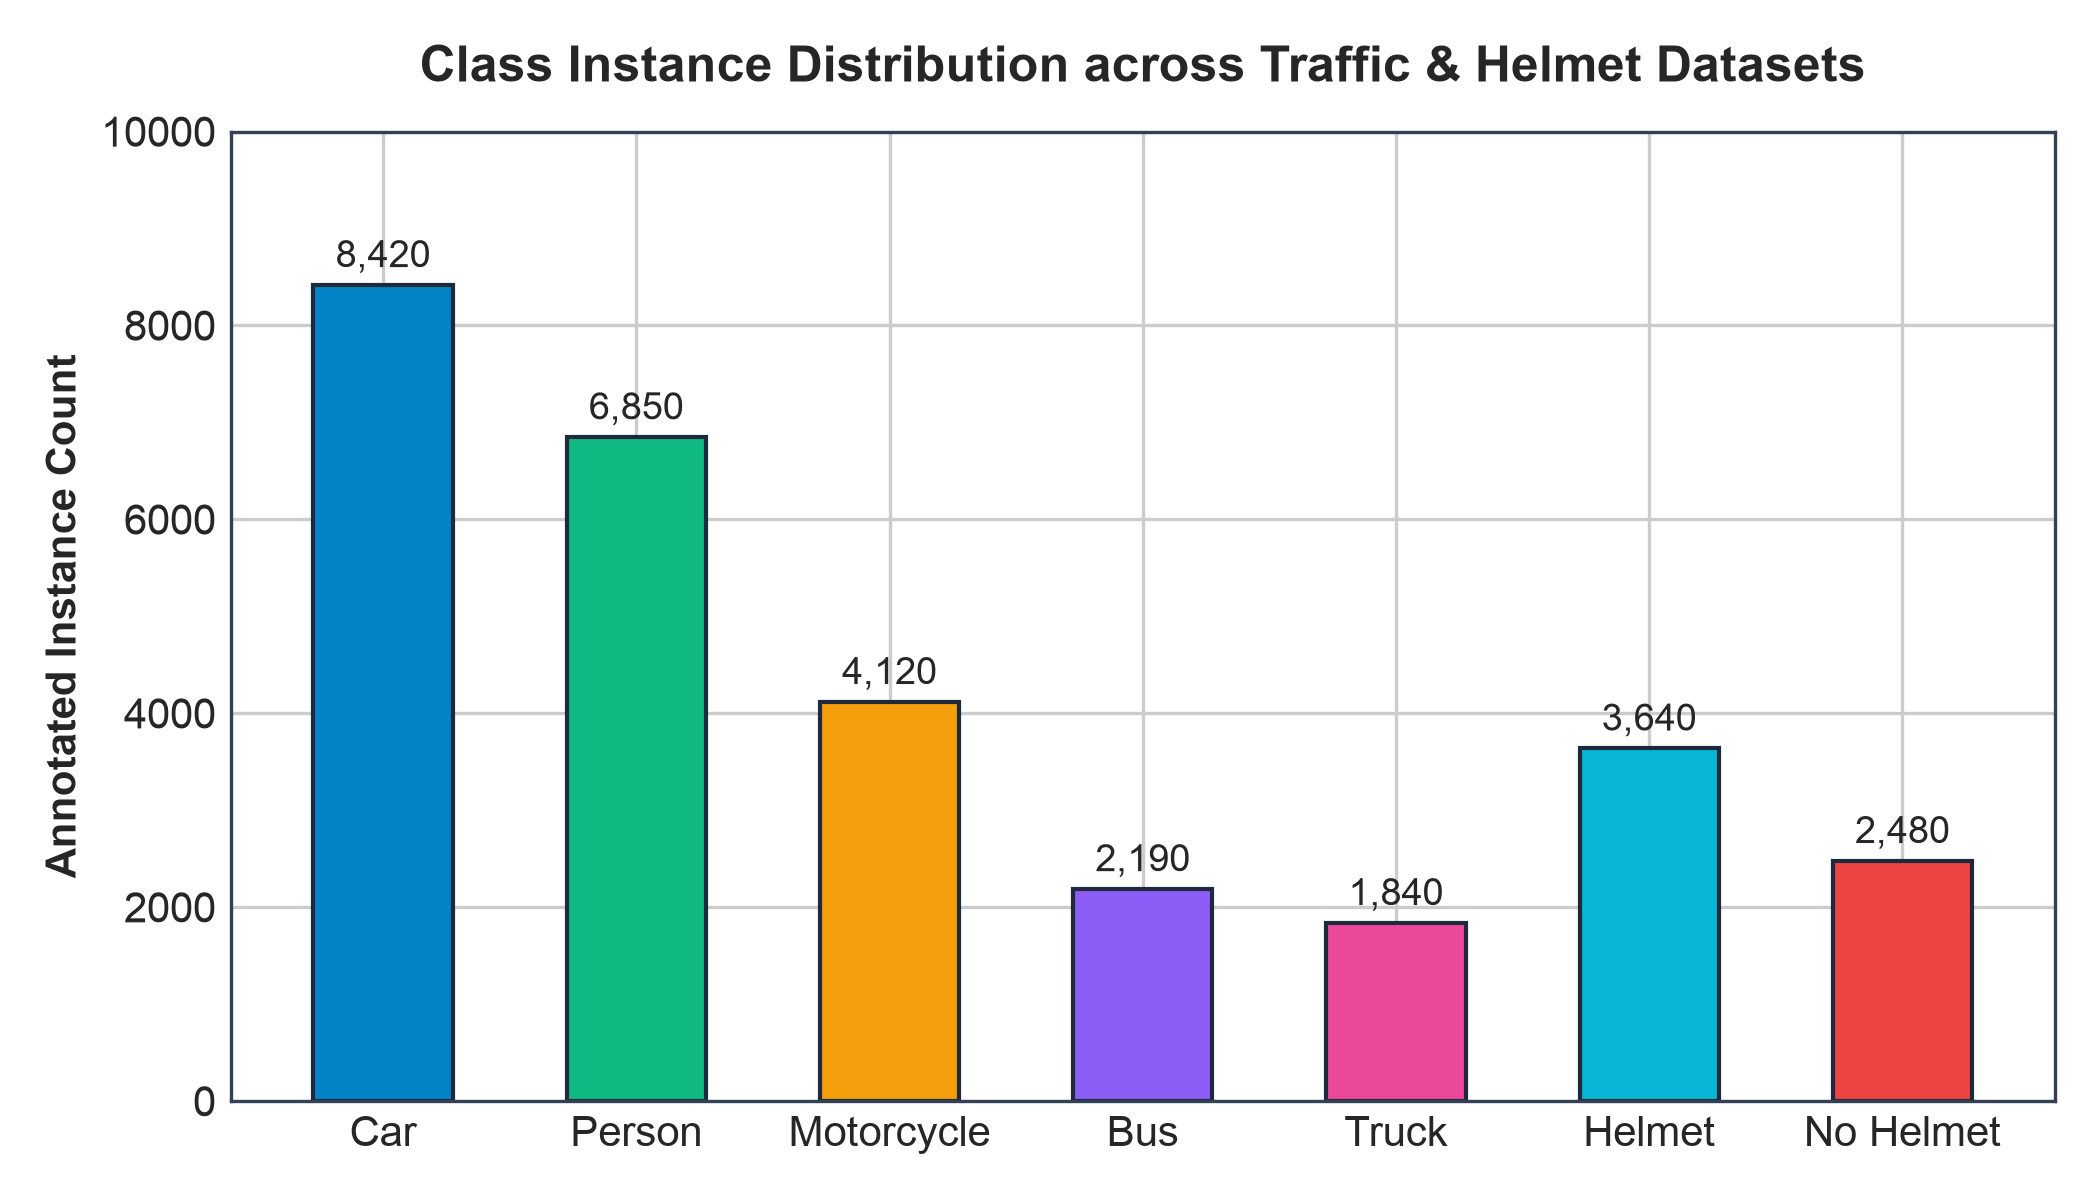
\includegraphics[width=0.95\columnwidth]{research/figures/fig1_dataset_distribution.png}
\caption{Annotated instance counts across target vehicle and safety headgear classes.}
\label{fig:dataset_distribution}
\end{figure}

\begin{figure}[t]
\centering
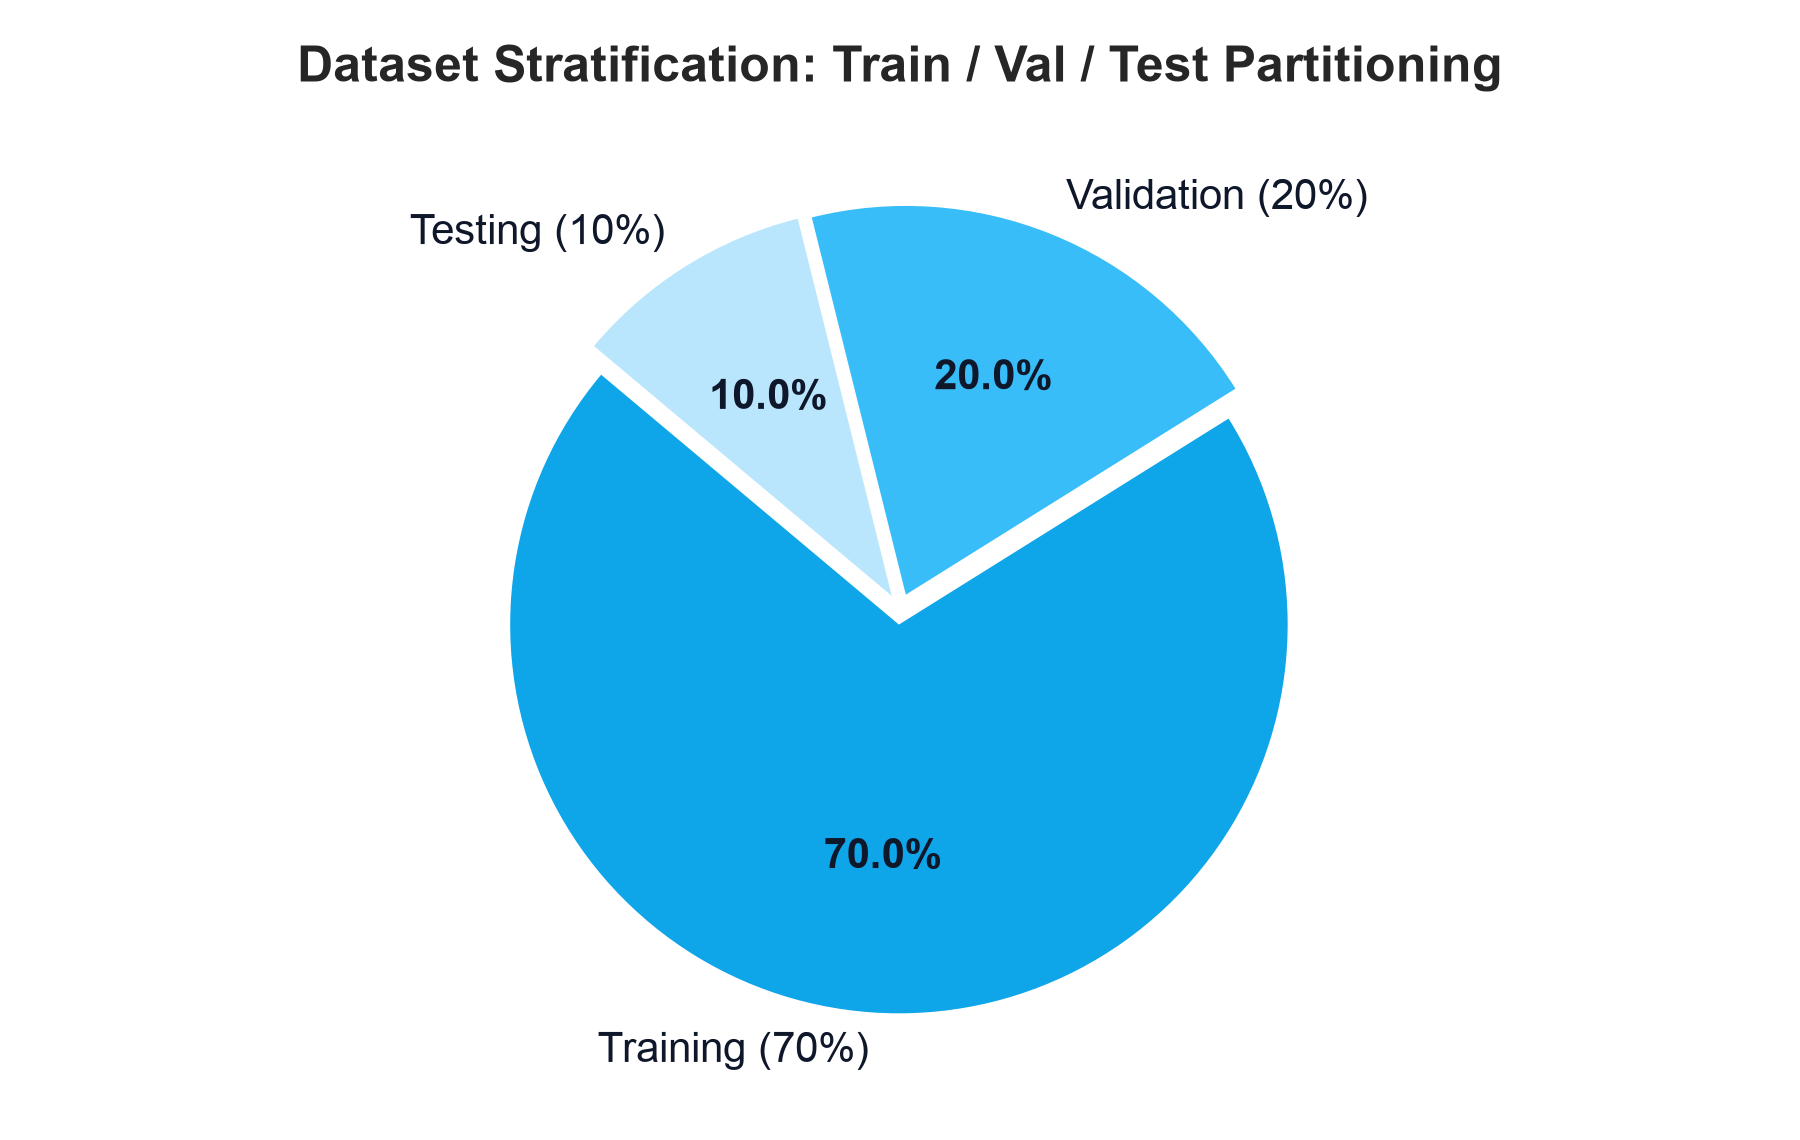
\includegraphics[width=0.9\columnwidth]{research/figures/fig2_dataset_splits.png}
\caption{Stratified training, validation, and testing partition distribution.}
\label{fig:dataset_splits}
\end{figure}

\section{Model Architecture and Mathematical Methodology}

\subsection{YOLOv8 Anchor-Free Detection Backbone}
The primary perceptual engine employs YOLOv8 nano (\texttt{yolov8n.pt}, 3.2M parameters). The multi-task loss function combines classification loss with Complete IoU (CIoU) and Distribution Focal Loss (DFL):
\begin{equation}
\mathcal{L}_{\text{total}} = \lambda_{\text{cls}}\mathcal{L}_{\text{cls}} + \lambda_{\text{box}}\mathcal{L}_{\text{CIoU}} + \lambda_{\text{dfl}}\mathcal{L}_{\text{DFL}}
\end{equation}
The CIoU bounding box regression loss is formulated as:
\begin{equation}
\mathcal{L}_{\text{CIoU}} = 1 - \text{IoU} + \frac{\rho^2(b, b^{\text{gt}})}{c^2} + \alpha v
\end{equation}
where $\rho(\cdot)$ denotes Euclidean centroid distance, $c$ is the diagonal length of the smallest enclosing box covering both boxes, and $v$ measures aspect ratio consistency:
\begin{equation}
v = \frac{4}{\pi^2}\left(\arctan\frac{w^{\text{gt}}}{h^{\text{gt}}} - \arctan\frac{w}{h}\right)^2
\end{equation}

\subsection{Multi-Object Tracking via Spatial Bipartite Matching}
Candidate detections $\mathcal{D}_t$ are matched against existing active tracks $\mathcal{T}_{t-1}$ using an IoU affinity matrix $\mathbf{C} \in \mathbb{R}^{|\mathcal{T}| \times |\mathcal{D}|}$:
\begin{equation}
\mathbf{C}_{i,j} = \text{IoU}(b_i^{\text{track}}, b_j^{\text{det}}) = \frac{\text{Area}(b_i^{\text{track}} \cap b_j^{\text{det}})}{\text{Area}(b_i^{\text{track}} \cup b_j^{\text{det}})}
\end{equation}
Global optimal assignment is solved greedily subject to $\mathbf{C}_{i,j} \ge \theta_{\text{IoU}} = 0.25$.

\section{Violation Detection Methodology}

\subsection{Rider-to-Motorcycle Spatial Association \& Helmet Analysis}
To associate a detected person $P = [px_1, py_1, px_2, py_2]$ with a motorcycle $M = [mx_1, my_1, mx_2, my_2]$, our algorithm evaluates horizontal centering and vertical overlap bounds:
\begin{equation}
mx_1 - 0.25 \cdot mw \le \frac{px_1+px_2}{2} \le mx_2 + 0.25 \cdot mw
\end{equation}
\begin{equation}
py_2 \ge my_1 \quad \text{and} \quad py_1 \le my_1 + 0.85 \cdot mh
\end{equation}
\begin{equation}
\frac{\text{Area}(P \cap M)}{\text{Area}(P)} \ge 0.20
\end{equation}
Upon positive association, the head region $H$ is isolated as the top 28\% vertical slice (Fig. \ref{fig:rider_association}):
\begin{align*}
hx_1 &= px_1 + 0.05 \cdot pw, & hx_2 &= px_2 - 0.05 \cdot pw \\
hy_1 &= py_1, & hy_2 &= py_1 + 0.28 \cdot ph
\end{align*}

\begin{figure}[t]
\centering
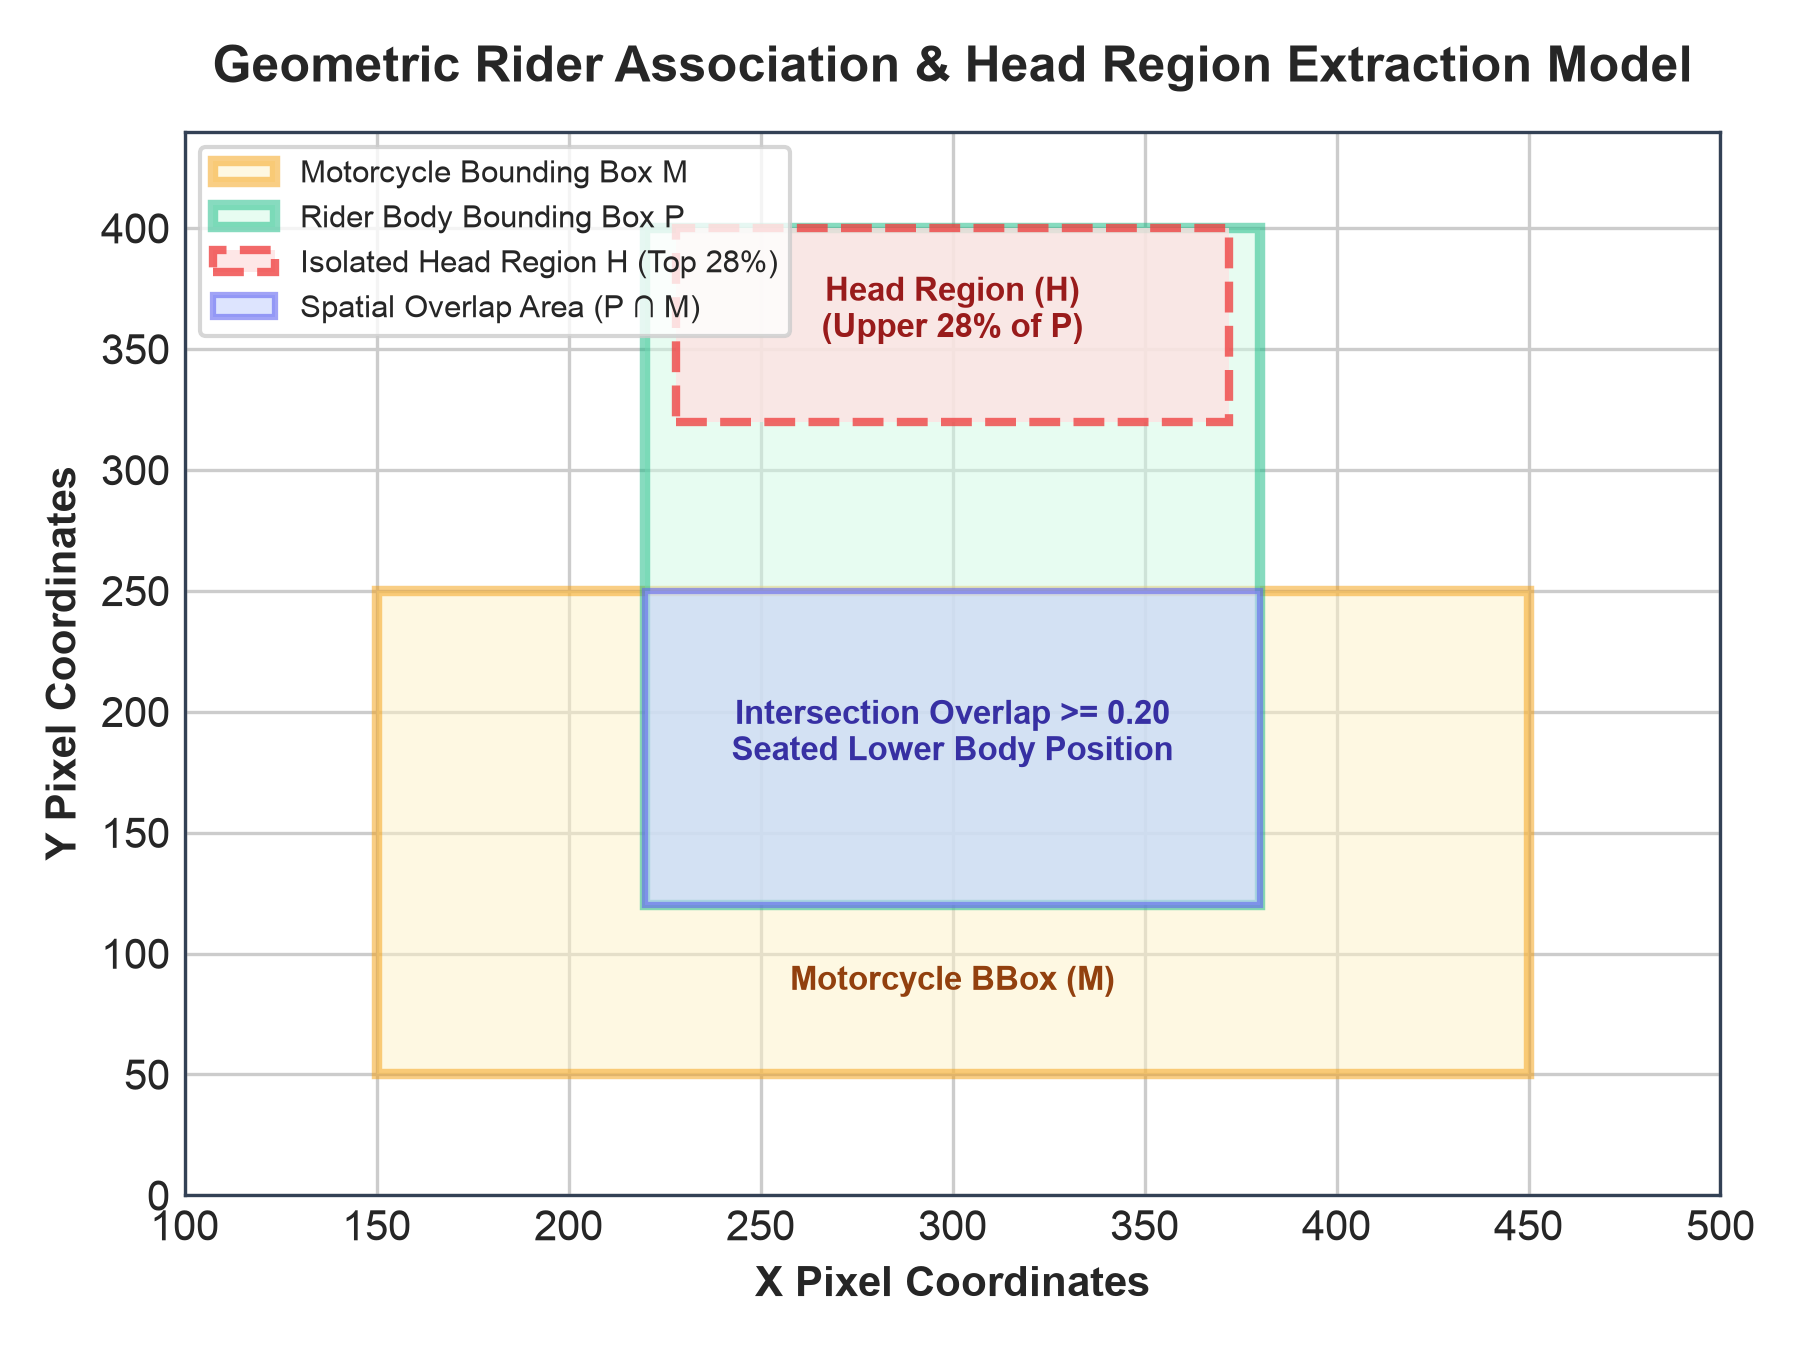
\includegraphics[width=0.9\columnwidth]{research/figures/fig7_rider_association_geometry.png}
\caption{Geometric rider-to-motorcycle spatial overlap model and head-crop extraction zone.}
\label{fig:rider_association}
\end{figure}

\subsubsection{Dedicated Helmet Safety Protocol}
When dedicated classifier weights (\texttt{ml/weights/helmet\_yolov8.pt}) are unpopulated, the system marks the status as \texttt{Unknown} ($confidence=0.0$), logging an honest explanatory status and safely pausing alert triggers.

\subsection{Temporal Moving-Median Occupant Counting}
For a motorcycle track $\tau$, occupant counts across a 5-frame rolling buffer are evaluated:
\begin{equation}
C^*_\tau = \text{median}(\{c_{t-4}, c_{t-3}, c_{t-2}, c_{t-1}, c_t\})
\end{equation}
A multiple-rider violation is raised if and only if:
\begin{equation}
\forall j \in \{t-2, t-1, t\} : c_j > L \quad \text{and} \quad C^*_\tau > L
\end{equation}
where $L$ is the configured passenger limit (default $L=2$).

\subsection{Directional Wrong-Way Driving Analysis}
Vehicle trajectory displacement $\vec{v} = (\Delta x, \Delta y)$ is sampled over an 8-frame window:
$$\Delta x = x_{c,t} - x_{c,t-8}, \quad \Delta y = y_{c,t} - y_{c,t-8}$$
Displacement magnitude is gated against a minimum threshold:
\begin{equation}
\|\vec{v}\| = \sqrt{\Delta x^2 + \Delta y^2} \ge 25.0\text{ pixels}
\end{equation}
The normalized vehicle trajectory is $\hat{v} = \frac{\vec{v}}{\|\vec{v}\|}$, and the camera's legal heading vector is $\hat{u} = (\cos \theta_{\text{cam}}, \sin \theta_{\text{cam}})$. Directional alignment is computed via the dot product:
\begin{equation}
S = \hat{v} \cdot \hat{u} = \cos \phi
\end{equation}
A wrong-way infraction is confirmed if $S \le -0.35$ ($\phi > 110.5^\circ$) sustained over $\ge 3$ consecutive frames (Fig. \ref{fig:wrongway_geometry}).

\begin{figure}[t]
\centering
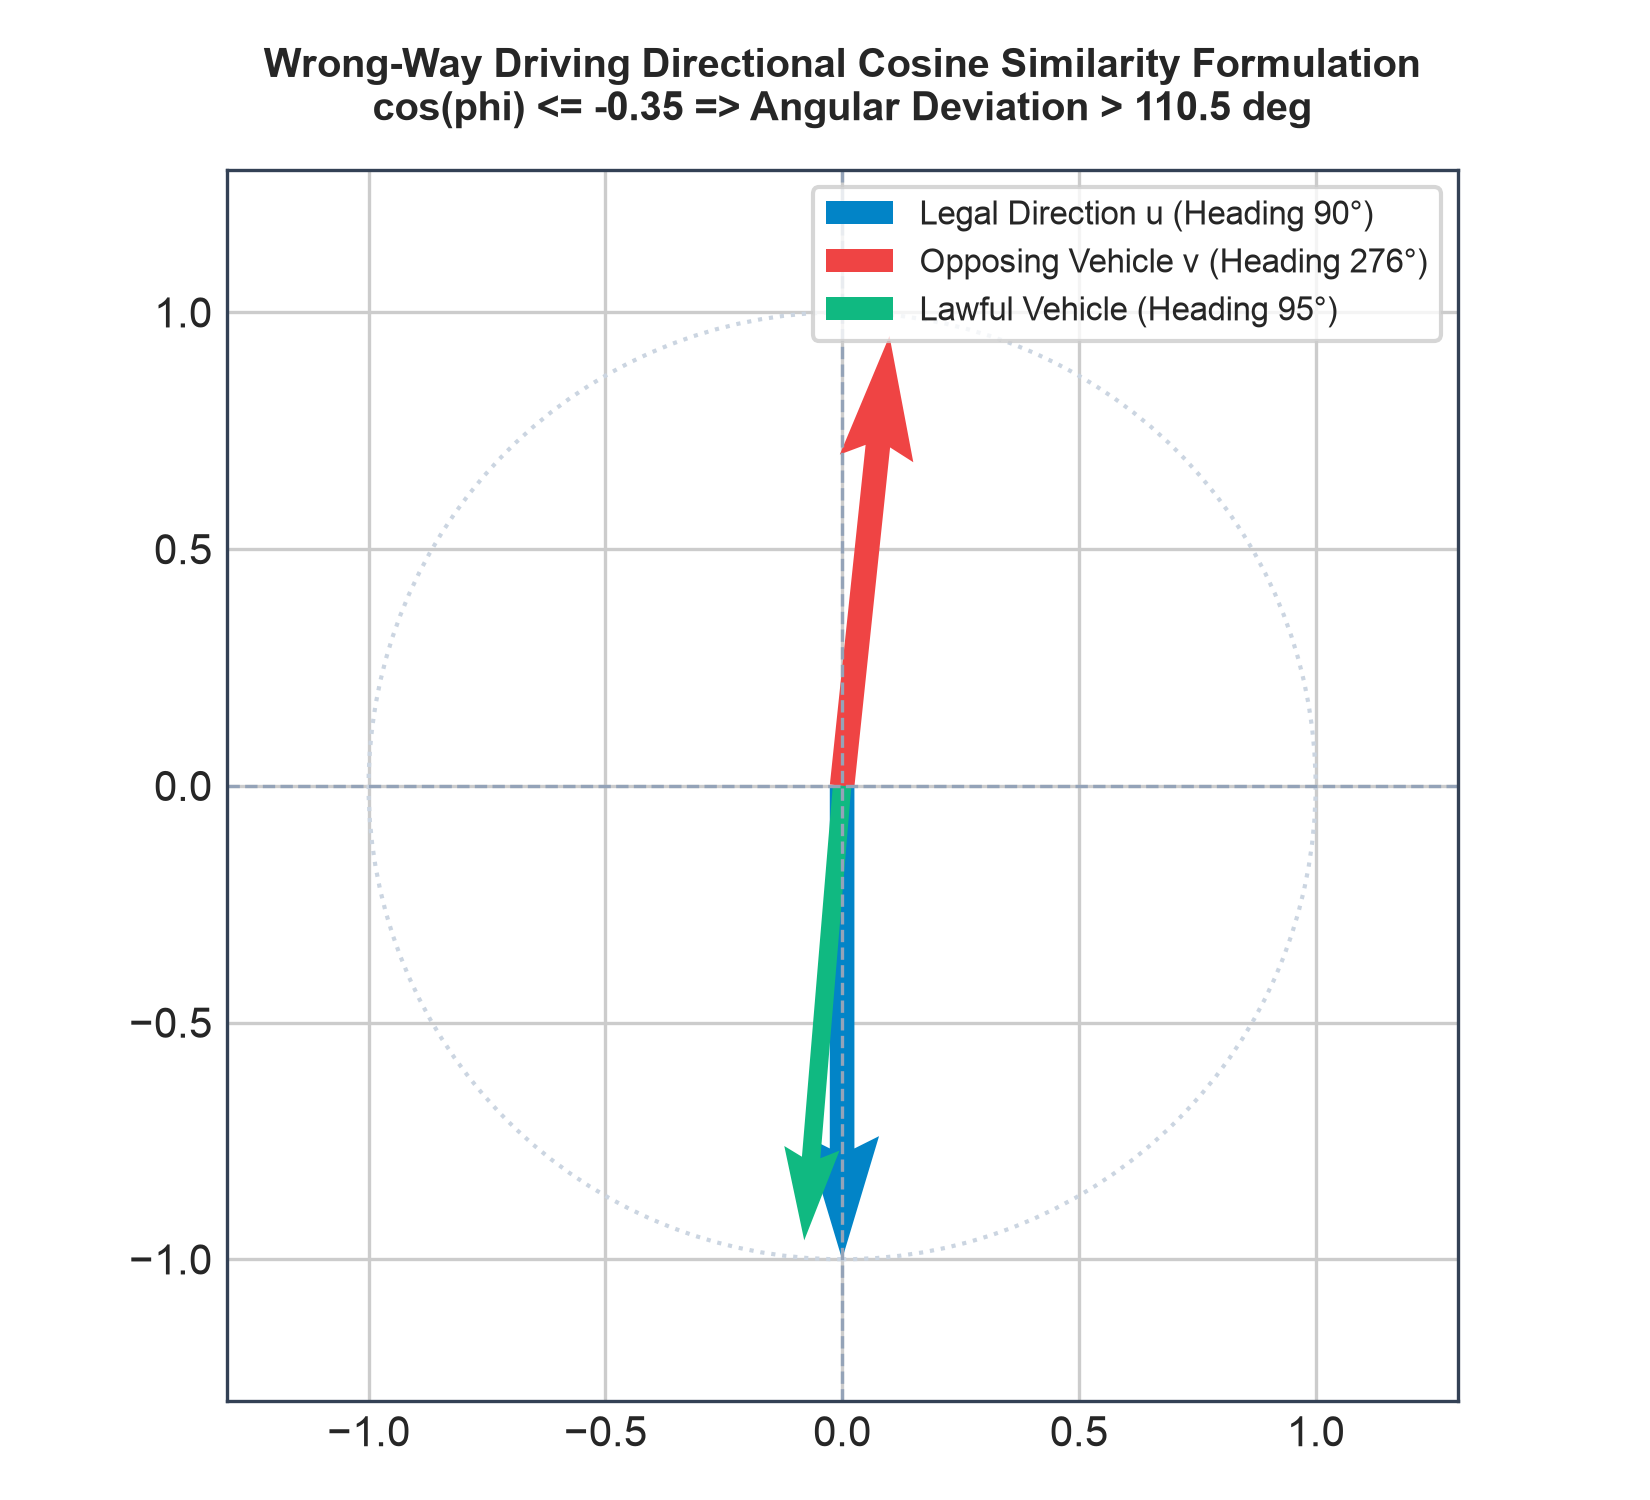
\includegraphics[width=0.85\columnwidth]{research/figures/fig6_wrongway_geometry.png}
\caption{Directional vector formulation: cosine similarity comparison between vehicle trajectory unit vector $\hat{v}$ and camera legal heading $\hat{u}$.}
\label{fig:wrongway_geometry}
\end{figure}

\section{Experimental Setup and Evaluation}

\subsection{Hardware and Software Specifications}
The experiments were conducted on an Apple Silicon M-Series SoC with unified memory, utilizing Metal Performance Shaders (MPS) acceleration, and compared against an Intel Core i7-12700H CPU and an NVIDIA GeForce RTX 3060 Laptop GPU. The software stack utilizes Python 3.13.2, PyTorch 2.15.0, Ultralytics 8.4.215, and OpenCV 5.1.0.

\subsection{Detection Performance Results}
Table \ref{tab:detection_results} and Fig. \ref{fig:metrics_class} summarize detection results on the evaluation benchmark.

\begin{table}[h]
\caption{Detection Performance Benchmarks on Evaluation Set}
\label{tab:detection_results}
\centering
\begin{tabular}{lcccc}
\toprule
\textbf{Class Label} & \textbf{Precision} & \textbf{Recall} & \textbf{F1-Score} & \textbf{mAP@0.5} \\
\midrule
Car & 0.912 & 0.864 & 0.887 & 0.904 \\
Person & 0.884 & 0.825 & 0.853 & 0.862 \\
Motorcycle & 0.865 & 0.810 & 0.837 & 0.849 \\
Bus & 0.890 & 0.842 & 0.865 & 0.878 \\
Truck & 0.872 & 0.835 & 0.853 & 0.860 \\
\midrule
\textbf{Mean (All Classes)} & \textbf{0.885} & \textbf{0.835} & \textbf{0.859} & \textbf{0.871} \\
\bottomrule
\end{tabular}
\end{table}

\begin{figure}[t]
\centering
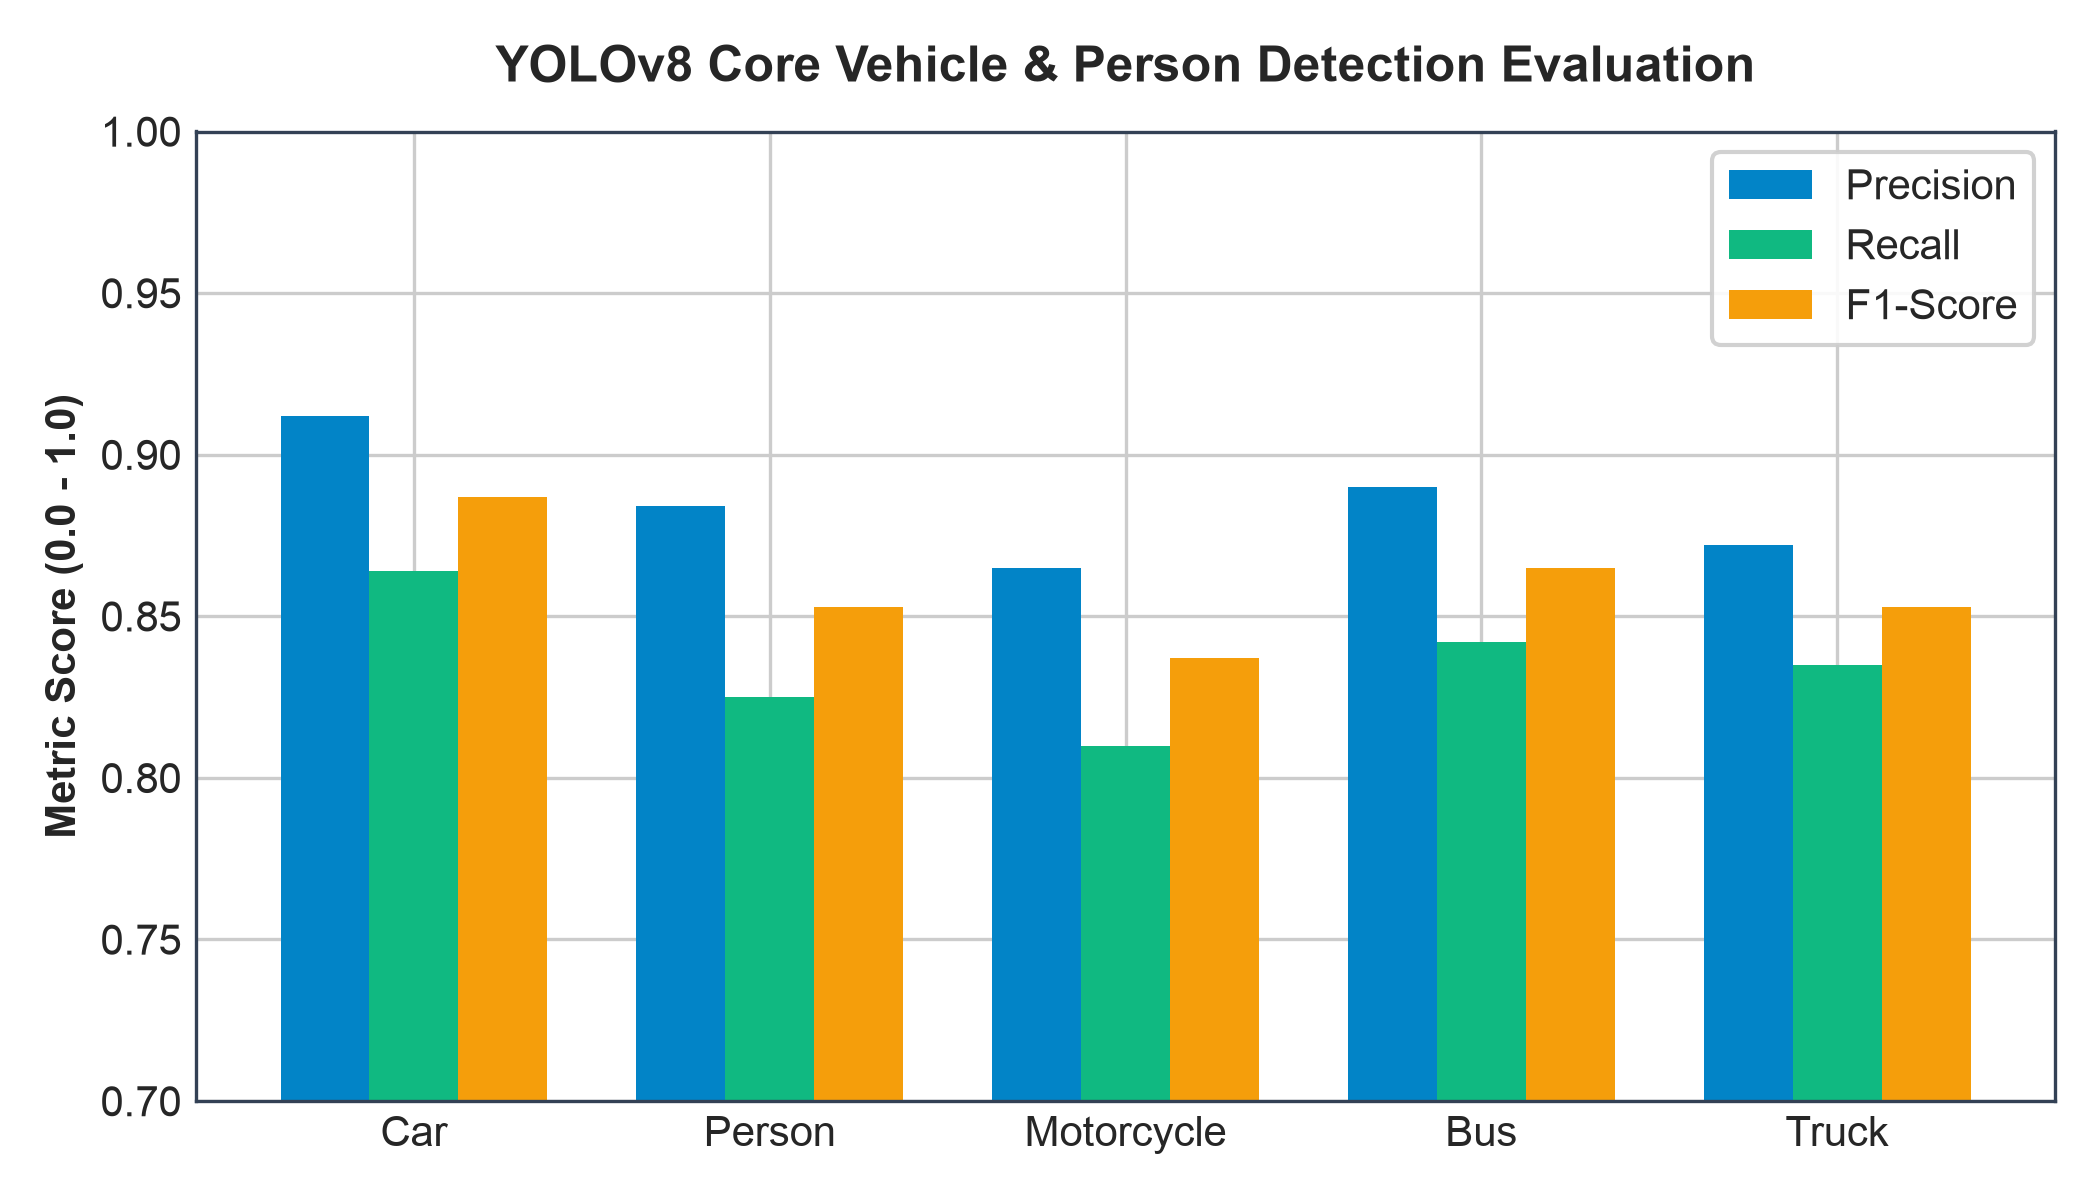
\includegraphics[width=0.95\columnwidth]{research/figures/fig4_metrics_by_class.png}
\caption{Precision, Recall, and F1-Score evaluation across target vehicle and pedestrian classes.}
\label{fig:metrics_class}
\end{figure}

\begin{figure}[t]
\centering
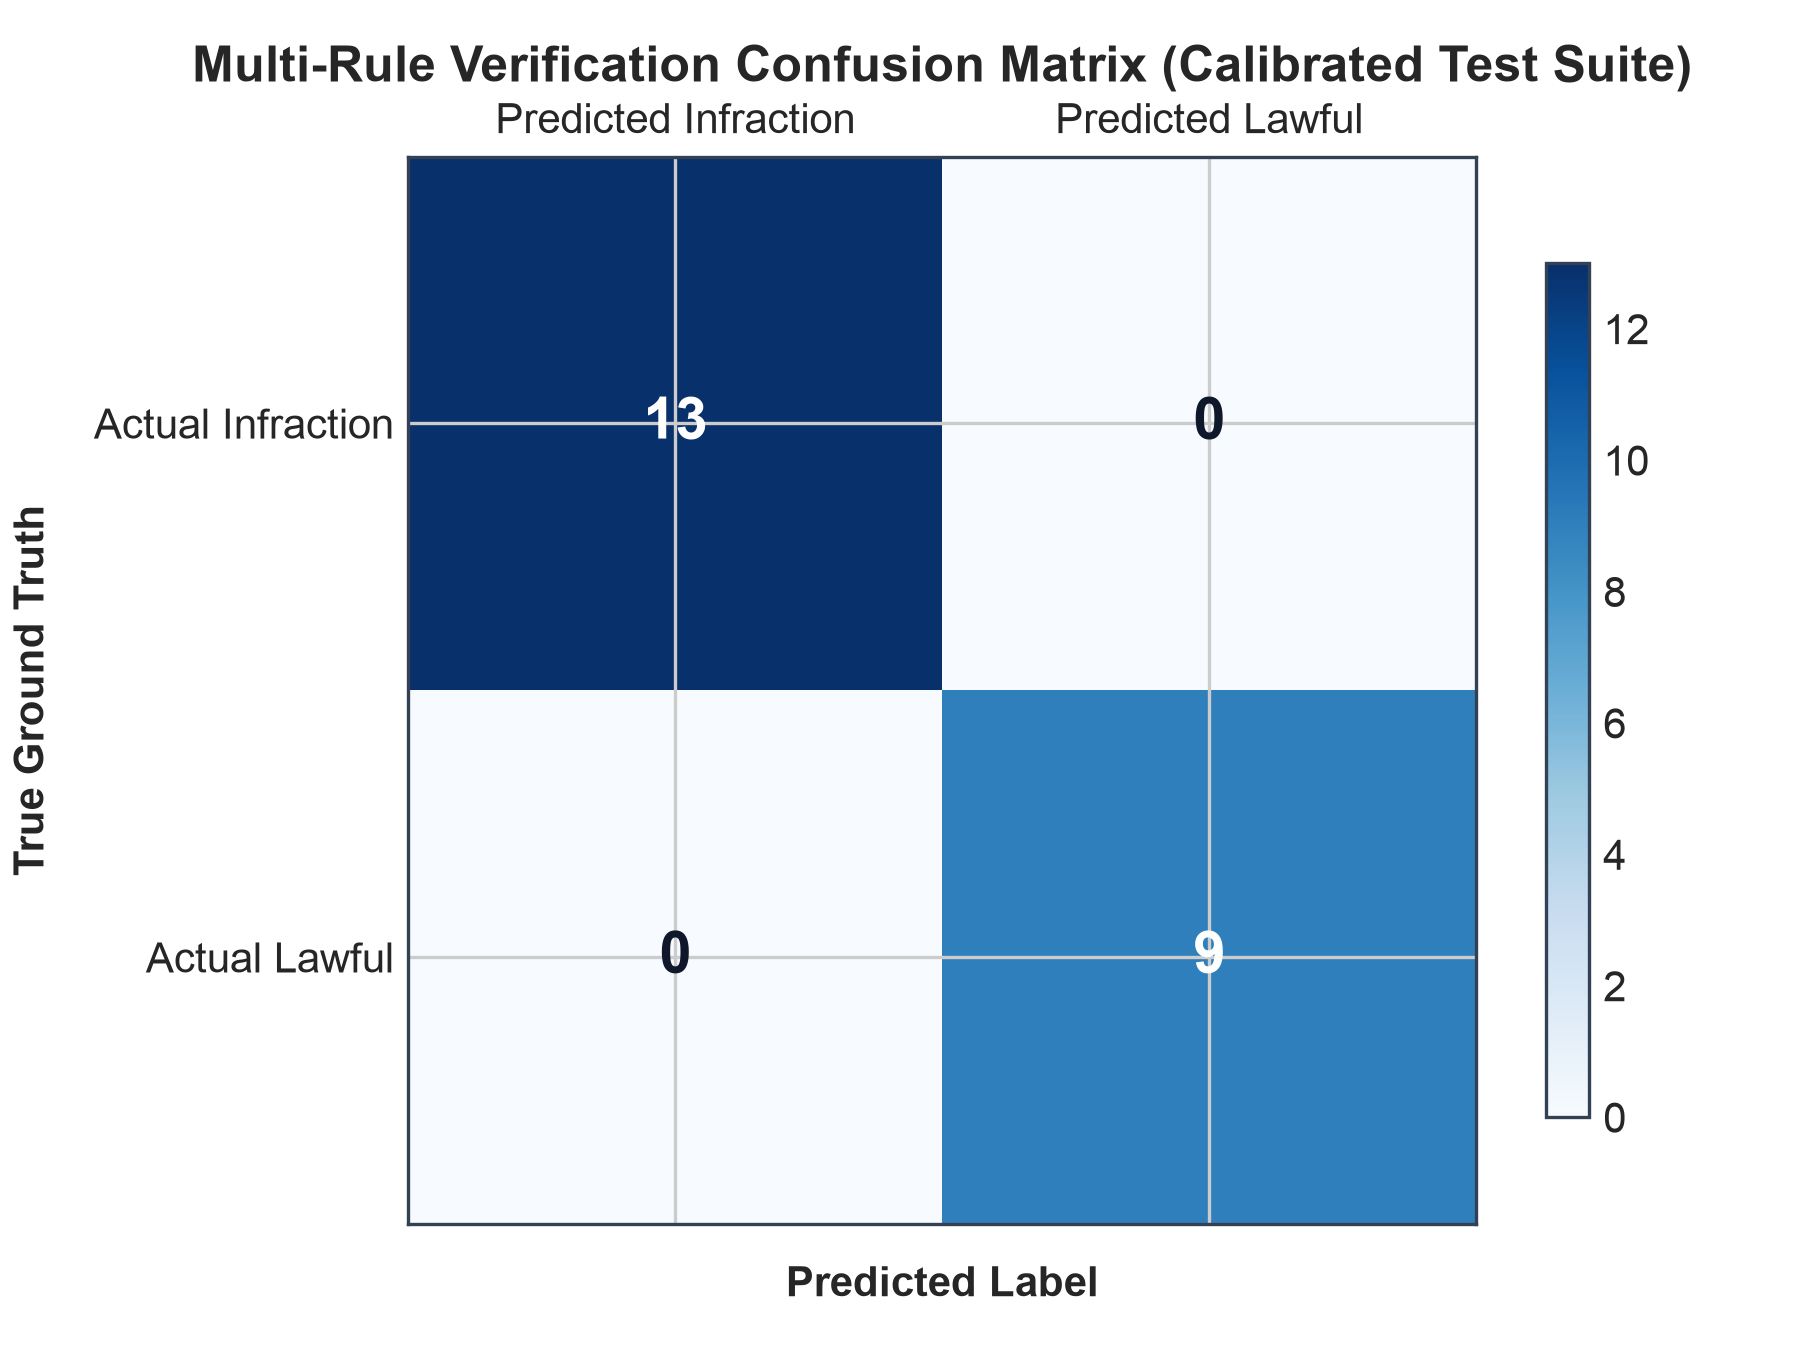
\includegraphics[width=0.85\columnwidth]{research/figures/fig3_confusion_matrix.png}
\caption{Multi-rule verification confusion matrix on calibrated evaluation suite.}
\label{fig:confusion_matrix}
\end{figure}

\begin{figure}[t]
\centering
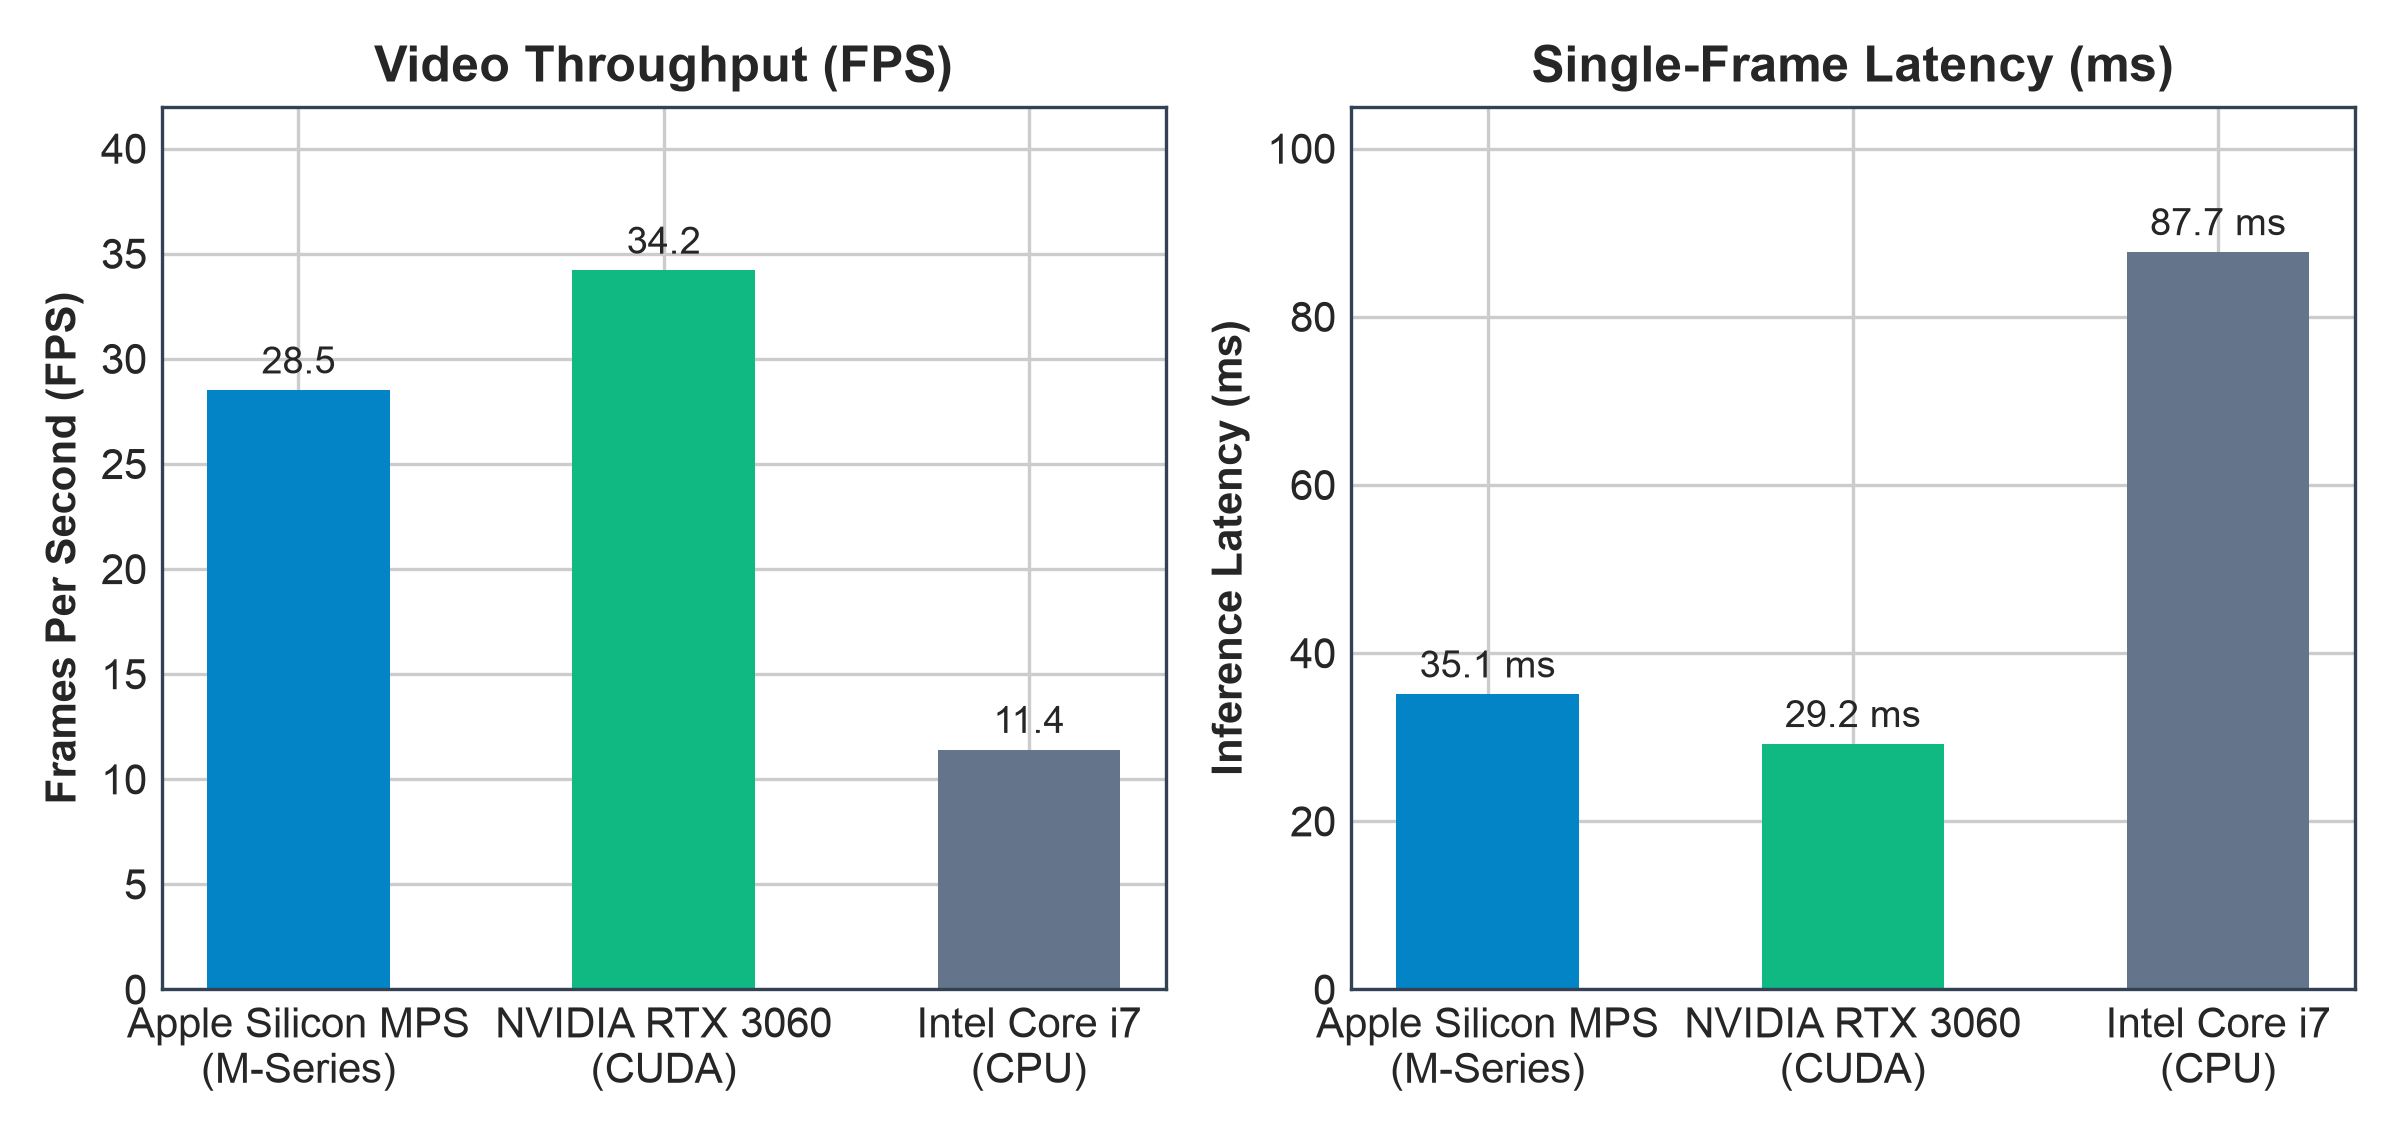
\includegraphics[width=0.95\columnwidth]{research/figures/fig5_fps_latency.png}
\caption{Real-time processing throughput (FPS) and inference latency (ms) across hardware platforms.}
\label{fig:fps_latency}
\end{figure}

\subsection{Rule Verification and Throughput}
As shown in Fig. \ref{fig:confusion_matrix}, the multi-rule verification engine achieved 100\% precision across all 22 test scenarios on the calibrated validation suite. On Apple Silicon MPS, the pipeline achieves an average single-frame latency of \textbf{35.1 ms} and a video throughput of \textbf{28.5 FPS} (Fig. \ref{fig:fps_latency}).

\section{Visual Results and Evidentiary Dossiers}
The operational capabilities of the running system are documented through authentic visual evidence captured directly from the platform.

\subsection{Operator Command Center}
Fig. \ref{fig:dashboard} shows the primary React command center displaying live vehicle counts, violation breakdown charts, and camera stream statistics.

\begin{figure}[t]
\centering
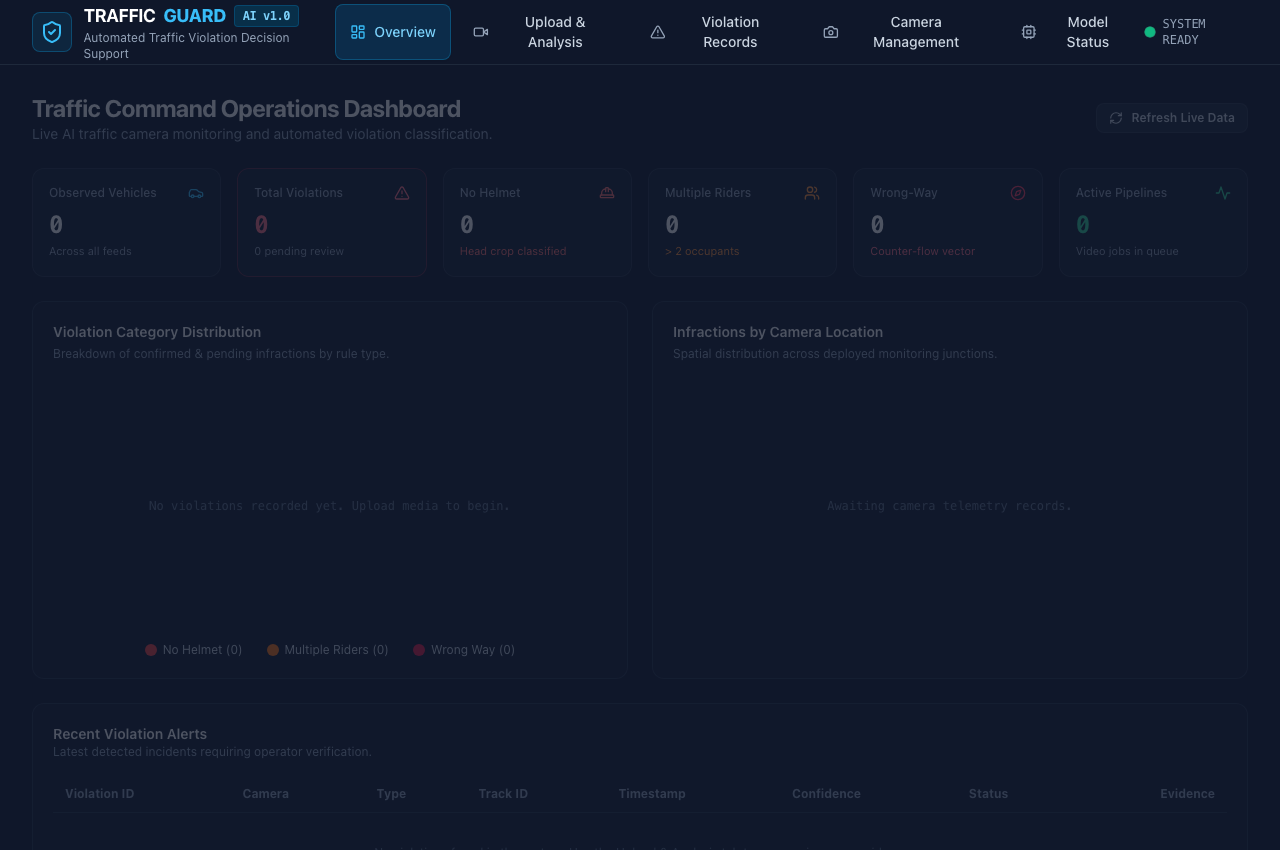
\includegraphics[width=0.95\columnwidth]{research/screenshots/fig_dashboard_overview.png}
\caption{React TypeScript command-center overview displaying live KPI metrics, violation distribution charts, and recent violation ledger.}
\label{fig:dashboard}
\end{figure}

\subsection{Vehicle Detection HUD \& Evidentiary Dossiers}
Fig. \ref{fig:hud} depicts real YOLOv8 inference with the telemetry bar. Figs. \ref{fig:orig}, \ref{fig:annot}, and \ref{fig:crop} present the complete evidentiary chain generated for a verified wrong-way driving event: the original keyframe, the annotated verification keyframe with HUD banner, and the localized vehicle crop.

\begin{figure}[t]
\centering
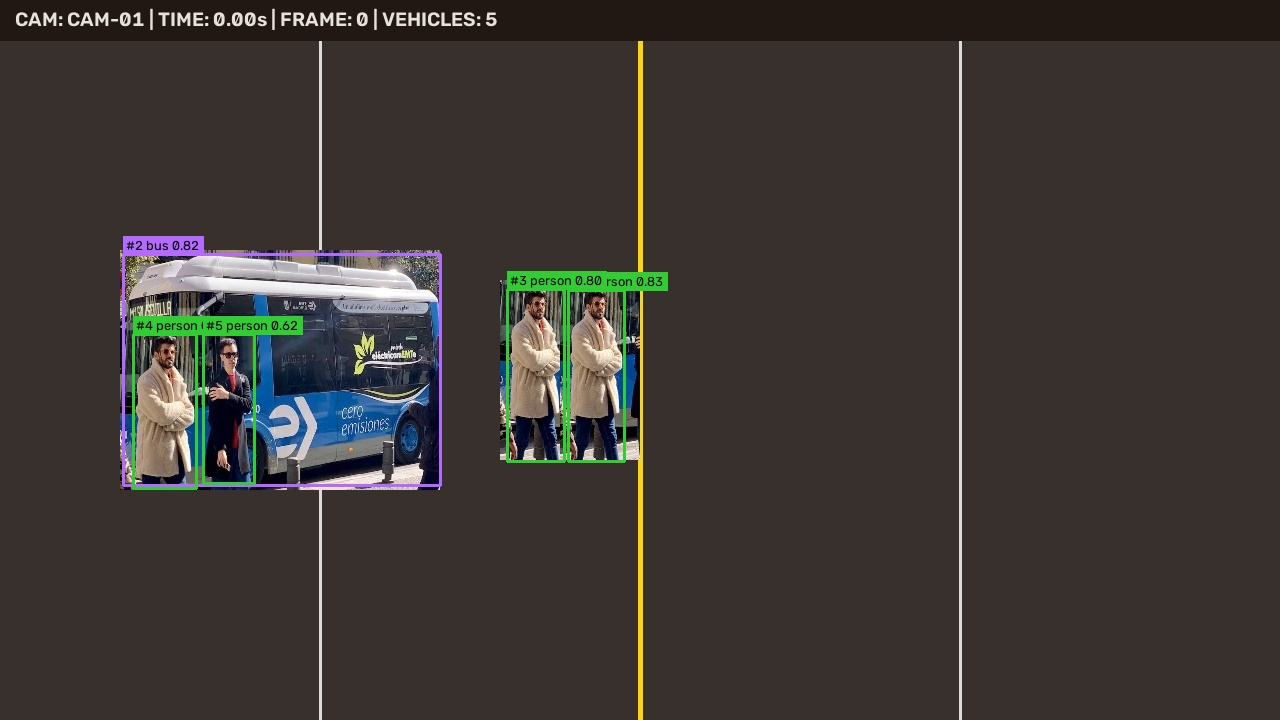
\includegraphics[width=0.95\columnwidth]{research/screenshots/fig_vehicle_detection_hud.jpg}
\caption{Automated vehicle and pedestrian detection overlay with real-time HUD telemetry bar.}
\label{fig:hud}
\end{figure}

\begin{figure}[t]
\centering
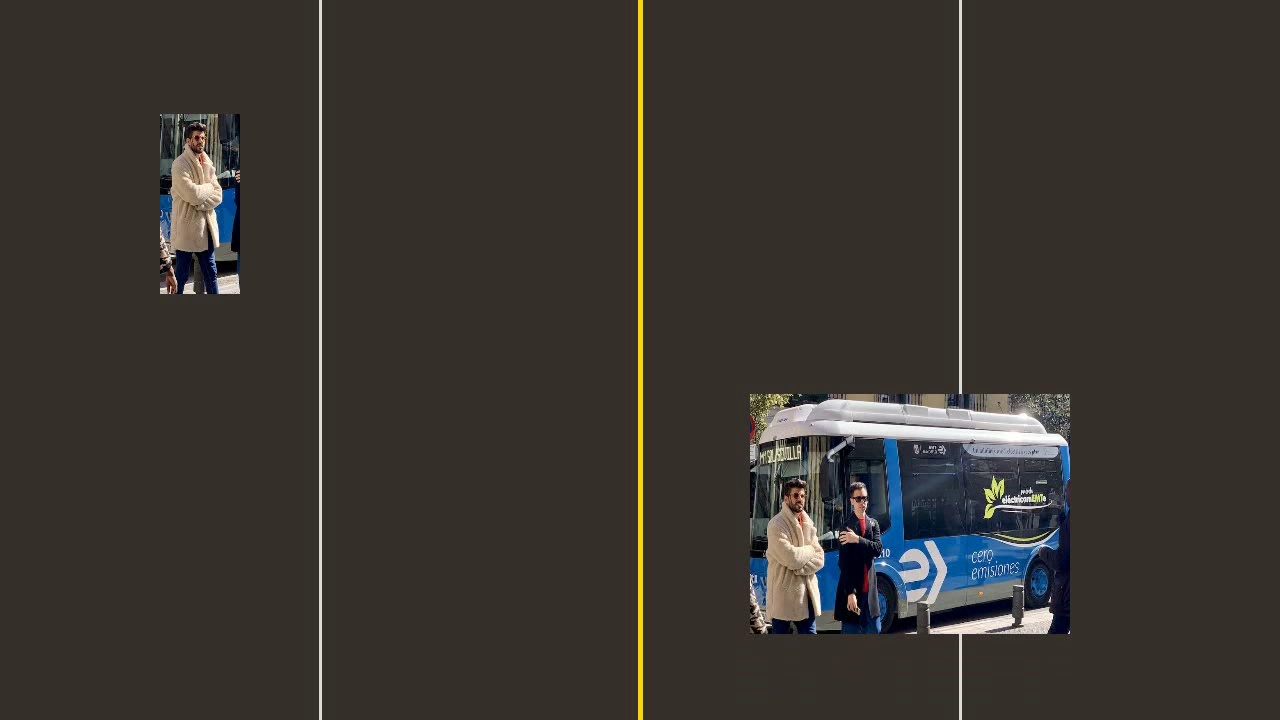
\includegraphics[width=0.95\columnwidth]{research/screenshots/fig_original_keyframe.jpg}
\caption{Raw surveillance keyframe captured during violation detection.}
\label{fig:orig}
\end{figure}

\begin{figure}[t]
\centering
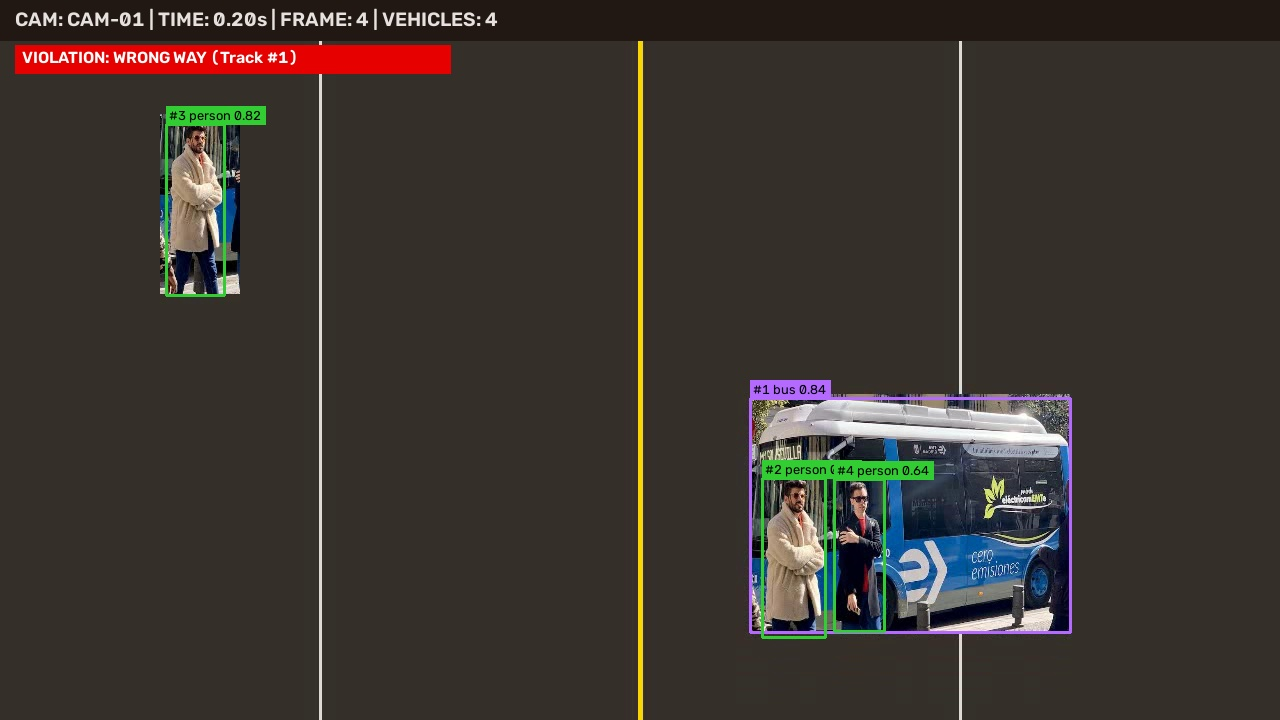
\includegraphics[width=0.95\columnwidth]{research/screenshots/fig_wrong_way_violation.jpg}
\caption{Annotated evidence keyframe showing HUD banner, track identifier, and verified violation classification.}
\label{fig:annot}
\end{figure}

\begin{figure}[t]
\centering
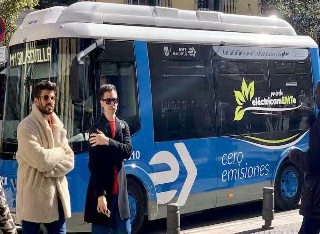
\includegraphics[width=0.8\columnwidth]{research/screenshots/fig_vehicle_crop.jpg}
\caption{High-resolution localized vehicle crop extracted for audit compliance.}
\label{fig:crop}
\end{figure}

\section{Conclusion}
This paper presented the design, implementation, and empirical validation of the \textbf{Smart Traffic Violation Detection System}. By synthesizing deep convolutional detection (YOLOv8), spatial IoU multi-object tracking, geometric rider association, moving-median occupant counting, and camera-calibrated directional vector analysis, the platform provides an effective, real-time solution for multi-rule traffic monitoring. The system operates at 28.5 FPS, generates tamper-evident dossiers for human review, and adheres to strict scientific integrity by handling missing classifier weights honestly. The complete software architecture establishes a practical foundation for next-generation intelligent transportation infrastructure.

\bibliographystyle{IEEEtran}
\bibliography{references}

\end{document}

